
\chapter{Data Sources}
  \label{ch:datasources}

  \section{A collection of skies}
    This work relies completely on all-sky surveys. All of the maps utilized are photometric-band infrared maps, except for the AME data, which is an all-sky component separation analysis product, from the Planck Collaboration's efforts to separate galactic foregrounds from the CMB. Table~\ref{tab:data} summarizes the observational data used in this thesis.
    \begin{table}[h]
      \caption{Observational data sources used in this article}
      \centering
        \begin{tabular}{lrrrrr}
        \hline\hline
        Instrument & Central Wavelength & FWHM & Cali & Reference \\
        \hline
        AKARI/IRC & 9~$\mu$m  &  \textasciitilde{}10$"$ & \textless 10\%   & \tablefootnote{\cite{ishihara10}} \\
        AKARI/IRC & 18~$\mu$m & \textasciitilde{}10$"$  & \textless 10\%     & '' \\
        AKARI/FIS & 65~$\mu$m  & 63$"$ & \textless 10\% & \tablefootnote{\cite{doi15,takita16}} \\
        AKARI/FIS & 90~$\mu$m  & 78$"$ & \textless 10\%   & '' \\
        AKARI/FIS & 140~$\mu$m & 88$"$ & \textless 10\%   & '' \\
        AKARI/FIS & 160~$\mu$m & 88$"$ & \textless 10\%   & '' \\
        IRAS/IRIS & 12~$\mu$m   & 4.0$'$ &   \textless 5.1\%       & \tablefootnote{\cite{iris05}} \\
        IRAS/IRIS & 25~$\mu$m   & 4.0$'$ &    \textless 15.1\%      & ''\\
        IRAS/IRIS & 60~$\mu$m   & 4.2$'$ &    \textless 10.4\%      & '' \\
        IRAS/IRIS & 100~$\mu$m  & 4.5$'$ &   \textless 13.5\%       & '' \\
        Planck/HFI & 345~$\mu$m & 4.7$'$ & & \tablefootnote{\cite{hfi14viii}} \\
        Planck/HFI & 550~$\mu$m & 4.3$'$& & '' \\
        \hline
         \label{tab:data}
      \end{tabular}
    \end{table}
    In total, we employ all-sky maps from 12 photometric bands, spanning the wavelength range of 6.9~$\mu$m to 550~$\mu$m as showin in Fig.~\ref{fig:Filter_coverage_example_full} The following sections give the details of the observational data from each instrument as well as of the parameter maps provided in \cite{planck15X}.\footnote{Planck bands are named according to their central frequency, not wavelength.}
      \begin{figure}
        \centering
        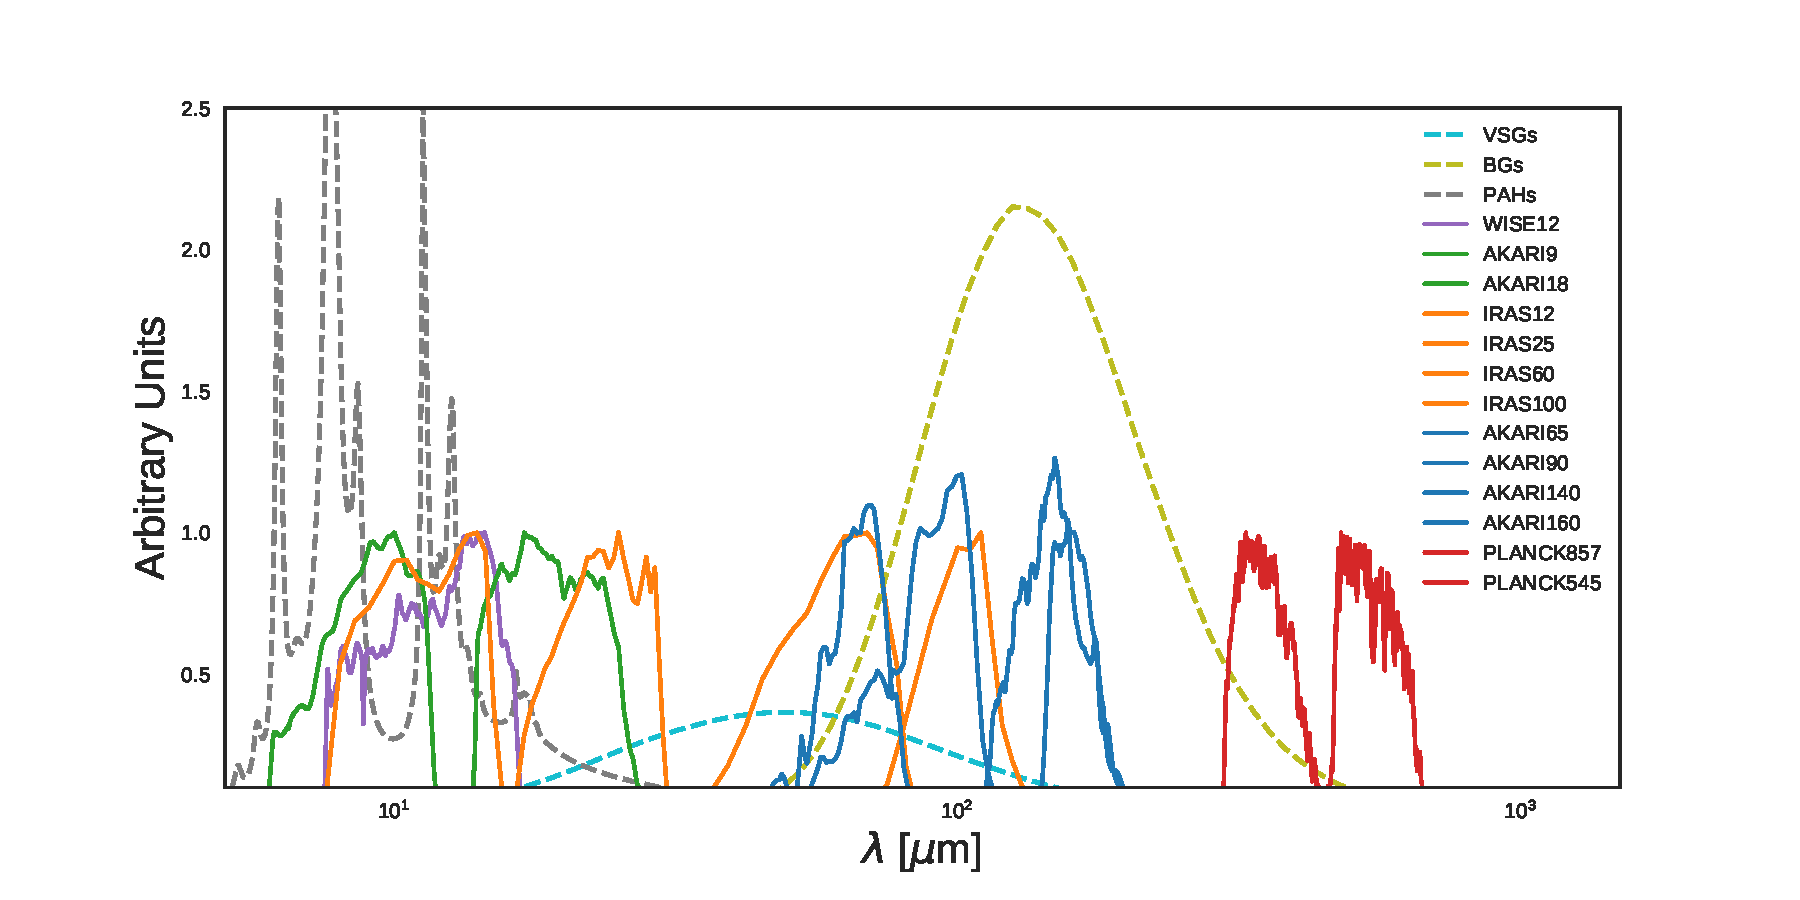
\includegraphics[width=\textwidth]{../Plots/ch_datasources/Filter_coverage_example_full.pdf}
        \caption{Relative spectral response curves of the bands used in this study. Expected dust emission components, assuming the dust SED model by \citep{dustem11} are also shown. The components are summarized as emission from big grains (BGs, dashed yellow line), emission from very small grains (VSGs, dashed blue line), and emission from PAHs (dashed grey line).}
        \label{fig:Filter_coverage_example_full}
      \end{figure}
    From this point in the thesis, we will mostly use abbreviations to refer to the different bands, as follows: 'A' indicates AKARI; 'D', DIRBE; 'I', IRAS, and 'P' Planck. The number after each letter indicates the band central nominal wavelength in microns (or frequency in GHz, in the case of the Planck bands.)
    \begin{table}[h]
      \caption{Ancilliary data}
      \centering
        \begin{tabular}{lrrrr}
        \hline\hline
        Product   & Relevant Freq./Wavelen  & FWHM    & Reference/URL \\
        \hline
        $H\alpha{}$  & 658.5~nm  & 36$'$  & \tablefootnote{\cite{finkbeiner03}: \url{https://lambda.gsfc.nasa.gov/product/foreground/halpha_map.cfm}} \\
        $N(H)$       & 21~cm     & 36$'$  & \tablefootnote{\cite{kalberla05}: \url{https://lambda.gsfc.nasa.gov/product/foreground/fg_LAB_HI_Survey_get.cfm}} \\
        PC $R$ (PR1)          & 353~GHz   & 5$'$   & \tablefootnote{\cite{}: \url{http://irsa.ipac.caltech.edu/data/Planck/release_1/all-sky-maps/previews/HFI_CompMap_ThermalDustModel_2048_R1.20/index.html} }\\
        PC $\tau_{353}$ (PR1) & 353~GHz   & 5$'$    & '' \\
        Haslam~MHz   & 408~MHz   & 56$'$  & \tablefootnote{\cite{haslam82}} \\
        PC Synchrotron (PR2) & 408~MHz & 60$'$ & \tablefootnote{\cite{planck15X}: \url{http://irsa.ipac.caltech.edu/data/Planck/release_2/all-sky-maps/previews/COM_CompMap_Synchrotron-commander_0256_R2.00/index.html}} \\
        PC $AME_{var}$ (PR2) & 22.8~GHz & 60$'$ & \tablefootnote{\url{http://irsa.ipac.caltech.edu/data/Planck/release_2/all-sky-maps/previews/COM_CompMap_AME-commander_0256_R2.00/index.html}} \\
        PC $AME_{fix}$ (PR2) & 41.0~GHz & 60$'$ & '' \\
        PC free-free (PR2) & N/A & 60$'$ & \tablefootnote{\url{http://irsa.ipac.caltech.edu/data/Planck/release_2/all-sky-maps/previews/COM_CompMap_freefree-commander_0256_R2.00/index.html}} \\
        \hline
         \label{tab:ancilliarydata}
      \end{tabular}
    \end{table}

  \section{AKARI}
  \label{sec:AKARI}
       The AKARI infrared space telescope revealed an entire sky of infrared light, from the mid to far infrared, via two instruments \citep{akari07} the Infrared Camera (IRC)\citep{irc07} and the Far Infrared Surveyor (FIS) \citep{fis07}. In this section we will discuss the all-sky surveys produced by these two instruments.
       \subsection{AKARI/Infrared Camera (IRC) }
           IRC proivded us with both spectroscopic and phometric data from the near to mid-infrared. In this work, we utilize the all-sky maps centered at 9 and 18~$\mu$m, created during by the IRC's fast-scanning mode. We utilize the most recent version of the IRC data (Ishihara, et al., in prep.) This version has had an updated model of the Zodiacal light, fitted and subtracted. The details of the improved Zodi-model, which offers an improvement over that used for the IRAS all-sky maps, are given in \cite{kondo16}.
       \subsubsection{PAH feature coverage}
         The A9 all-sky map demonstrates the abundance of the PAH bands carrier in the Milky Way \citep{ishihara10}. Figure~\ref{fig:Filter_coverage_example_PAH} shows the coverage of the PAH features (from both ionized and neutral PAH components), as they are theoretically determined in \cite{dustem11}.
            \begin{figure}
              \centering
              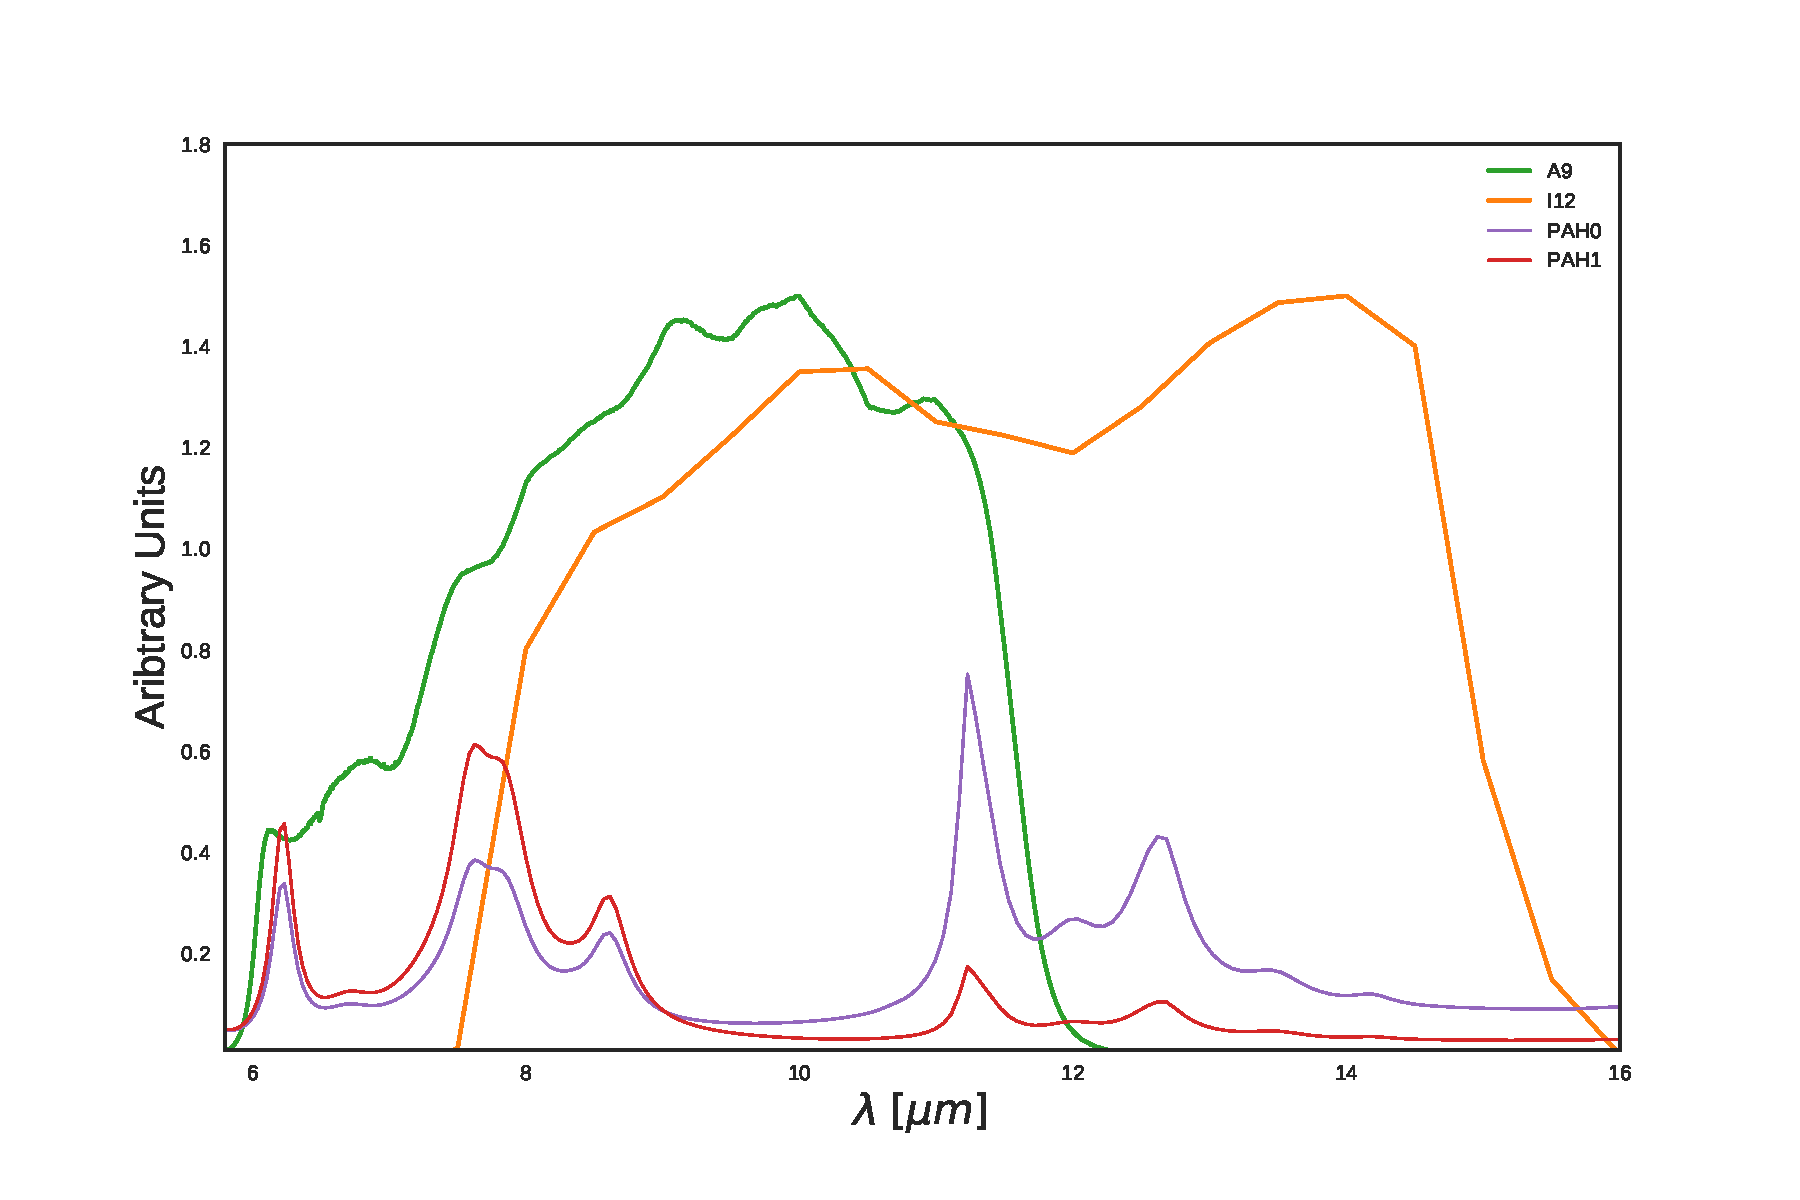
\includegraphics[width=\textwidth]{../Plots/ch_datasources/Filter_coverage_example_PAH.pdf}
              \caption{The I12 (orange) and A9 (green) filters coverage of modeled ionized (PAH1, red) and neutral (PAH0, purple)components of PAH features by \cite{dustem11}. The difference in the PAH feature coverage mainly comes from the 6.2~$\mu$m and the 7.7~$\mu$m feature.}
              \label{fig:Filter_coverage_example_PAH}
            \end{figure}
         The A9 band uniquely covers major ionized PAH features at 6.2 and 7.7~$\mu$m; as well as neutral PAH features at 8.6 and 11.2~$\mu$m across the entire sky \citep{irc07}. The I12 band covers the 11.2 and 8.6~$\mu$m features, and the similarly-shaped W12 band covers primarily the 11.2~$\mu{}$m feature but do not cover the 7.7~$\mu{}$m completely. According to the distribution of PAH features across the response filters in Fig.~\ref{fig:Filter_coverage_example_PAH}, and referring back to the various dust components in Fig.~\ref{fig:Filter_coverage_example_full} it is also expected that the A9 band is most dominated by PAH emission even with increasing $U$ . This may seem counter-intuitive, since, as described in Ch.~\ref{ch:intro}, the PAH spectral shape does not show a temperature variation. However as $T$ increases, the MIR extent of thermal dust emission and emission from VSGs encroach on I12 and WI2 sooner than A9, diluting emission from PAHs. In some ionized reigons, I12 may also include non-significant contributions from the [NeII] line at 12.8~$\mu$m. Figure~\ref{fig:Filter_coverage_example_MIR} demonstrates an example observational galactic cirrus spectrum in the MIR, from Spitzer Infrared Spectrograph (IRS) \citep{spitzer04} data, along with filters for all of the MIR bands used in this study.
             \begin{figure}
               \centering
               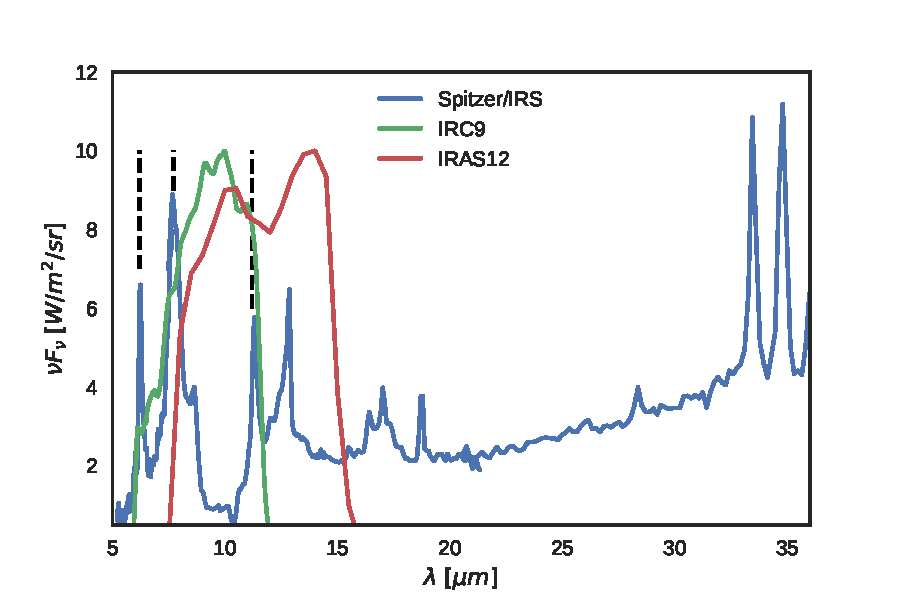
\includegraphics[width=\textwidth]{../Plots/ch_datasources/Filter_coverage_example_MIR.pdf}
               \caption{Coverage of MIR wavelengths by the filters used in this work. An Spitzer/IRS spectrum (see AOT4119040) of the galactic plane (thin blue line) demonstrates how IRC and IRAS photometric bands trace these features on an all-sky basis \citep{ishihara07}. Strong PAH features overlap with the A9 and I12, while the A18 and I25 micron bands only trace much weaker features. }
               \label{fig:Filter_coverage_example_MIR}
             \end{figure}
         It indicates that the other MIR bands, A18 and I25, do cover strong PAH features and are expected to be dominated rather by emission from very small grains (VSGs), as was indicated in Fig.~\ref{fig:Filter_coverage_example_full}.

         To help demonstate how the relative contribution from PAHs will change for each band, for different ISRF strengths, Fig.~\ref{fig:InBandFracContribution_PAH} gives just such a calculation. These contributions remain relatively constant out to a $U$ of about 100, with the contribution from warm dust becomming a larger factor for the I12 and W12 bands. Thus, according to the DL01 template, A9 should have the highest contribution from PAHs out to extreme radiation fields. At least to the extent with which PAHs can endure harsh UV radiation, as PAHs are expected to evaporate in strong enough radiation fields \citep{allain96a,allain96b,bocchio12,pilleri12, pavlyuchenkov13}.

      \subsubsection{PAH ionization}
        Figure~\ref{fig:Filter_coverage_example_PAH} indicates that expected emission from ionized PAHs may preferentially contribute to the A9 band, even though both I12 and A9 cover ionized and neutral features. A PAH SED model calculation, using the \cite{dustem11} SED template, supports that for Galactic cirrus ISM conditions, emisison detected by the A9 band would have a higher contribution from charged PAHs than the I12 band. This is demonstrated in Fig.~\ref{fig:InBandFracContribution_PAH}.
          \begin{figure}
              \centering
              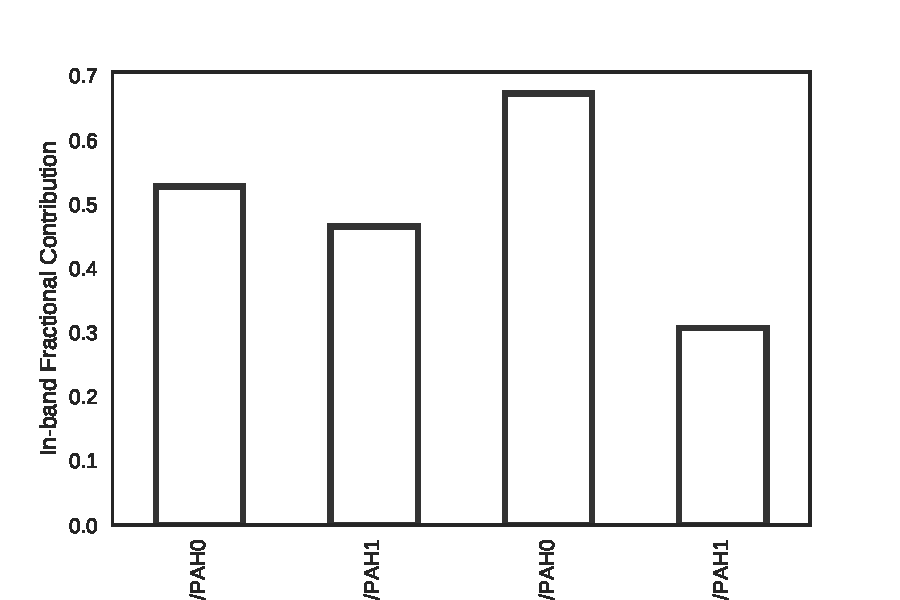
\includegraphics[width=\textwidth]{../Plots/ch_datasources/InBandFracContribution_PAH.pdf}
              \caption{In-band contributions from charged (PAH1) neutral (PAH0) PAHs, to the emission detected by the I12 and A9 filters. These assume a model galactic cirrus spectrum simulated with the SED template of \cite{dustem11}. }
              \label{fig:InBandFracContribution_PAH}
          \end{figure}
        To be clear, both bands are sensitive to both charged and neutral PAHs, however the relative contribution from charged PAHs is expected to be higher for A9. Thus we might expect that the ratio of intensities in this two bands, for a given line of sight (towards which PAHs are not destroyed), could trace the fraction of charged PAHs. Estimating the extent of this effect, Fig.~\ref{fig:band-ratio-multiple} gives the results of a calculation of I12/A9 and I25/A9 band ratios for two ISRF strengths.
          \begin{figure}
              \centering
              
\includegraphics[width=\textwidth]{../Plots/ch_datasources/band-ratio-multiple.pdf}
              \caption{Ionization fraction of PAHs vs. band ratios of I12, I25, to A9, for two ISRF strengths: Top: $U = 1$, Bottom: $U = 10$. These ratios are determined by assuming the SED template of \cite{dustem11} }
              \label{fig:band-ratio-multiple}
          \end{figure}
        This calculation is again based on \cite{dustem11}. It suggests that at least for $U<\sim{}10$, the fraction of charged PAHs may be estimated as a function of the I12/A9 ratio.

         Examing how this might look in the data themselves, Fig.~\ref{fig:ratioMap_A9I12} and Fig.~\ref{fig:ratioMap_A9I25} show the R(A9:I12) and R(A9:I25) ratio maps, demonstrating the relative variations in these MIR bands accross the sky--- or at least the portions of the sky where S/N is sufficient. While from visual inspection the various MIR intensity all-sky maps appear to essentially trace the same stuctures of the galaxy, the ratio maps reveal that there are indeed differences to be explored.  In regions where noise is dominant, ascertaining the ionization fraction will be quite difficult. This can be easily seen upon visual inspection of the ratio maps, in that there is a clear deliniation between brighter emission towards lower galactic latitudes, and the high latitude sky where the ratio shows very little discernible structure (except for the Zodi-residual patterns which differ between IRC and IRAS.) Thus there may a large portion of the sky where the S/N may be high enough to allow us to trace the PAH ionization fraction. This possibility is explored in Ch.~\ref{ch:lori}, in looking at the PAH distribution within $\lambda$~Orionis.
             \begin{figure}
               \centering
               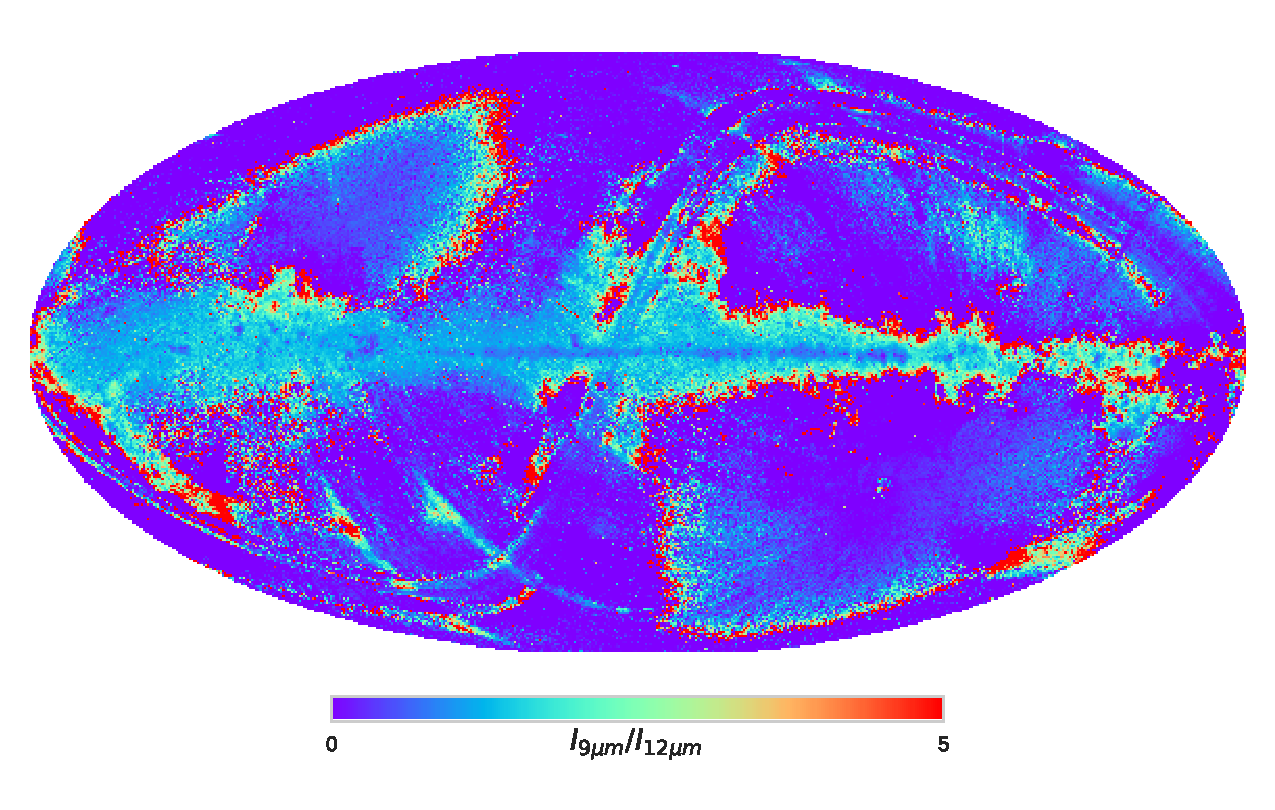
\includegraphics[width=\textwidth]{../Plots/ch_datasources/ratioMap_A9I12.pdf}
               \caption{ AKARI/IRC 9~$\mu$m to IRAS 12~$\mu$m intensity ratio.}
               \label{fig:ratioMap_A9I12}
             \end{figure}
             \begin{figure}
               \centering
               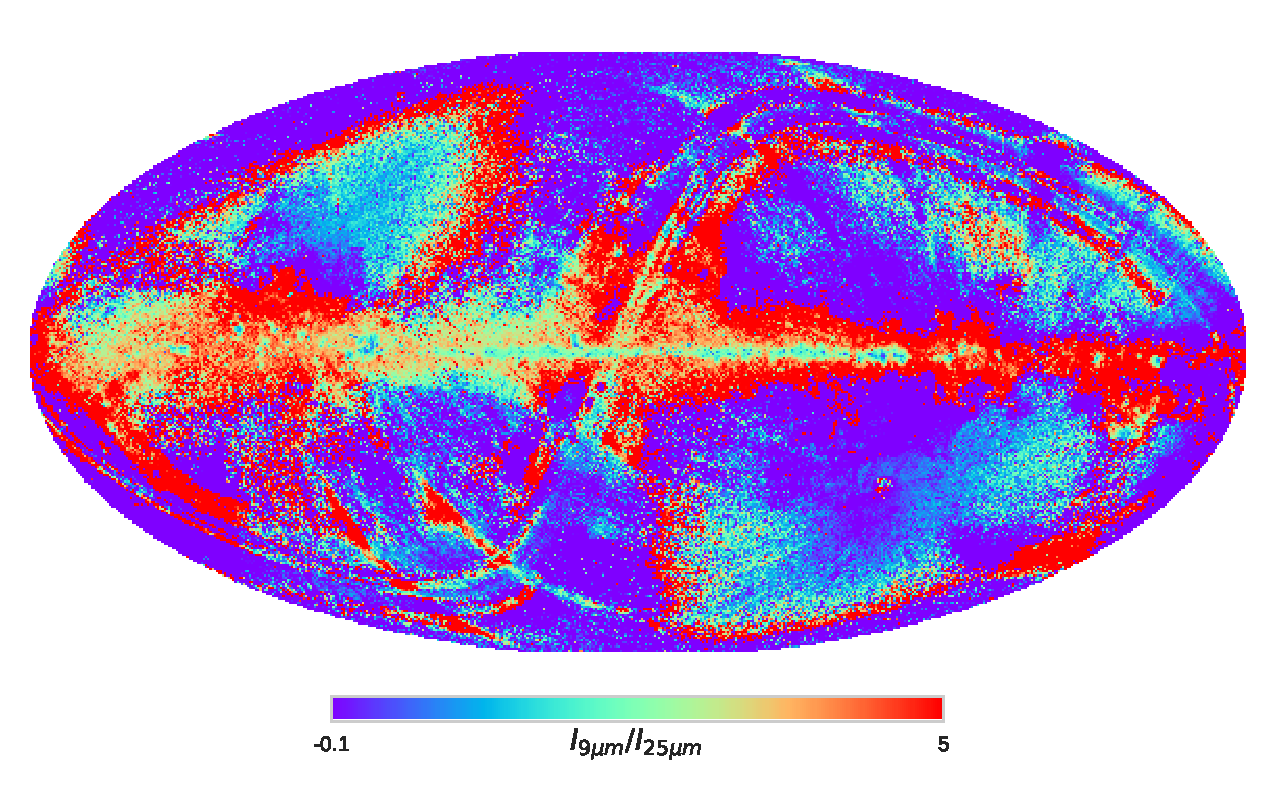
\includegraphics[width=\textwidth]{../Plots/ch_datasources/ratioMap_A9I25.pdf}
               \caption{ AKARI/IRC 9~$\mu$m to IRAS 25~$\mu$m intensity ratio.}
               \label{fig:ratioMap_A9I25}
             \end{figure}

    \subsection{The AKARI Far Infrared Surveyor (FIS)}
       FIS gives us photometric data around the peak of the typical thermal dust SED. FIS was equipped with four wavebands: two narrow bands centered at 65~$\mu$m and at 160~$\mu$m, and two wide bands at 90~$\mu$m and at 140~$\mu$m. An all-sky survey was carried out at each band \citep{kawada07}, and the processed maps have been publicly released \citep{doi15}.

    \subsection{Planck Observatory High Frequency Instrument (HFI)}
       The HFI all-sky maps, spanning 100 to 857~GHz \citep{hfi14viii} help constrain the far IR dust emissivity. This study utilizes the 857~GHz (345~$\mu$m) and 545~GHz (550~$\mu$m) bands.

    \section{Infrared Astronomical Satellite (IRAS)}
       Data from the IRAS \citep{iras84} all-sky surveys are used to supplement the similarly-centered AKARI photometric bands. The IRAS 12~$\mu$m band is similar to the IRC 9~$\mu$m band in terms of the sky coverage, central wavelength, and especially in that both surveys are heavily dominated by zodiacal light. We use the Improved Reprocessing of the IRAS Surveys (IRIS) \citep{iris05}, which have undergone a zodiacal-light removal. The zodiacal light model, however differs between the two bands. The IRAS zodi-subtraction is primarily based on the \cite{kelsall98} model, while IRC employs a modified version of this model \citep{kondo16}. Although WISE provides higher resolution than IRAS, we do not utilize the WISE data because we found the WISE all-sky 12~$\mu$m product to essentially trace the Planck HFI 857~GHz map, at 1$^{\circ}$ angular resolution. \cite{hensley16} had noted that this scaling of the WISE map may artificially suppress actual PAH-related variations at low resolution. Moreover, since we are conducting our analysis at 1$^{\circ}$ resolution in order to match the AME data, the higher resolution offered by WISE is not a significant advantage.

  \section{Planck COMMANDER Parameter Maps}
  \label{sec:PCmaps}
       We utilize the COMMANDER-Ruler astrophysical component separation maps \citep{planckXII}, from the Planck Collaboration's Public Data Release 2 (hereafter, PR2)\citep{planck2015I}. These contain estimates of known microwave foreground components (free-free, synchrotron, thermal dust emission contributions to the Planck photometric bands. Fig.~\ref{fig:PCCS_corrmatrix} demonstrates the correlatedness of these component maps, taken as provided in the PR2 archive.
         \begin{figure}
           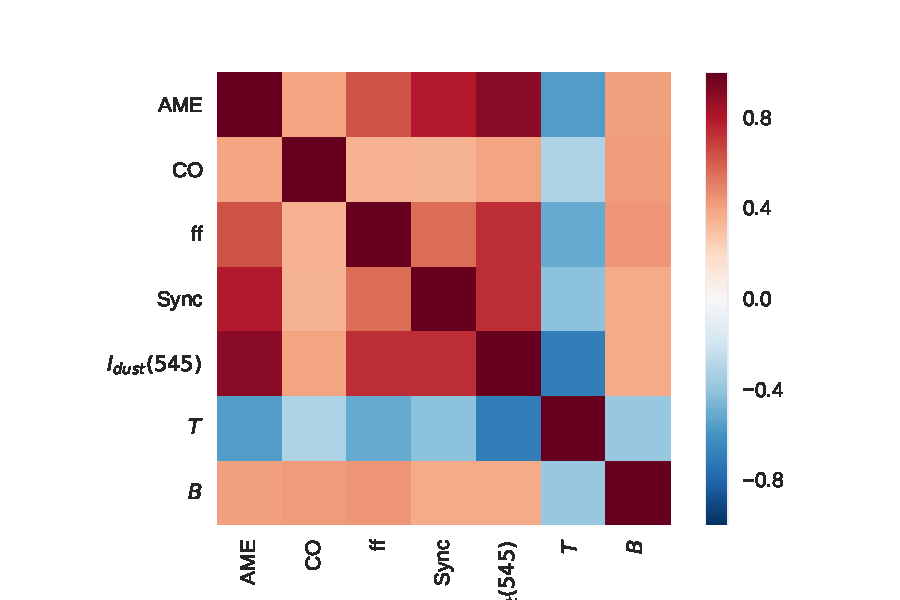
\includegraphics[width=\textwidth]{../Plots/ch_datasources/PCCS_corrmatrix.pdf}
           \centering
           \caption{$r_{s}$ cross correlation matrix of the PCCS maps: temperature $T$, emissivity index $\beta$, and amplitude at 545~GHz $I_{dust}(545)$ of thermal dust; intensity of free-free emission $ff$ at ; intensity of synchrotron emisison at 4~MHz $Sync$; intensity of the AME var. freq. component $AME$ at 22.8~GHz.}
           \label{fig:PCCS_corrmatrix}
         \end{figure}
        Without considering noise levels or variations of scale, we see evidence these major components are correlated with one another. In the case of free-free emission,  \cite{vonHausegger15} found that by taking S/N ratios into account, the correlation between COMMANDER free-free and AME components turns negative. More generally they suggest that the intercorrelations betwen these products varies with scale. We will first describe the 'non-AME' components, so as to not give any indiciation that their estimation is trival.

       \subsection{Synchrotron}
          While the Planck observations themselves do limit our resolution when assessing the AME - it is the primary constraint on synchrotron emission, 408~MHz map by \cite{haslam82} that is the major resolution limiting factor. While an impressive early effort to reveal the low-frequency sky, \citep{haslam82} is limited to an approximately 1$^{\circ}$ resolution. The map also contains many artifacts. For the time being however, it is still the most synchrotron-dominated all-sky map available, and for this reason PC15X included it in their COMMANDER component separation. Enhanced synchrotron mapping efforts are currently in progress by the `The final synchrotron product produced by COMMANDER (hereafter, PCSync) highly resembles the \cite{haslam82} map, however it is also demonstrated PCSync does not fully capture the synchrotron signal. This can be visualized by inspecting the PCAME:PCdust ratio map (see Fig.~\ref{fig:R_PCAMEtoPCdust}), which \cite{hensley16} describe as containing synchrotron emission patterns at high latitudes.

       \subsection{Free-free emission}
          Unlike the PCSync component, the fitting of the Planck COMMANDER free-free component map (hereafter, PCff) does not employ any free-free dominated emisison map, even though an earlier Planck AME paper \citep{planckXV} had employed the $H\alpha$ map by \cite{finkbeiner03}. Uncertainties in this map arise from uncertainties in the gas temperature, and the Gaunt factor. This emission source is the dominant source of confusion with AME, especially for HII regions \citep{planckXV,planckXII, paladini15}.

      \subsection{Thermal dust emission}
      ``Thermal dust emission'' in the COMMANDER context refers to dust emission in the Rayleigh Jeans-regime, as the COMMANDER fitting includes neither photometric constraints on the thermal emission peak, nor on Wiens-regime emission from small grains. This component essentially involves the fitting of a modified blackbody curve (Eq.~\ref{eq:mbb}.) to the Planck Photometry. This approach however results in an apparent anti-correlation between $\beta$ and $T$ (Fig.~\ref{fig:PCCS_corrmatrix}). Whether or not this anti-correltion is genuine is still unsettled in the literature \citep{galliano11,juvela12}. In any case, we do not utilize the $\beta$ and $T$, only the dust intensity at 545~GHz~($I_{d}$) parameter map.

      \subsection{AME data}
          The COMMANDER map release also provides an ``AME component map'', which presumes that AME originates from spinning dust. While acknowledging that such a decomposition lacks a strong physical interpretation, \cite{planck15X} break the AME into two components: a spatially varying peak frequency component, $AME_{var}$, and a spatially constant peak frequency component, $AME_{fix}$. As seen in Fig.~\ref{fig:AME_commander_freqdist}, virtually all of the fitted peak frequncies for $AME_{var}$ are beyond the reach of WMAP and Planck.
              \begin{figure}
                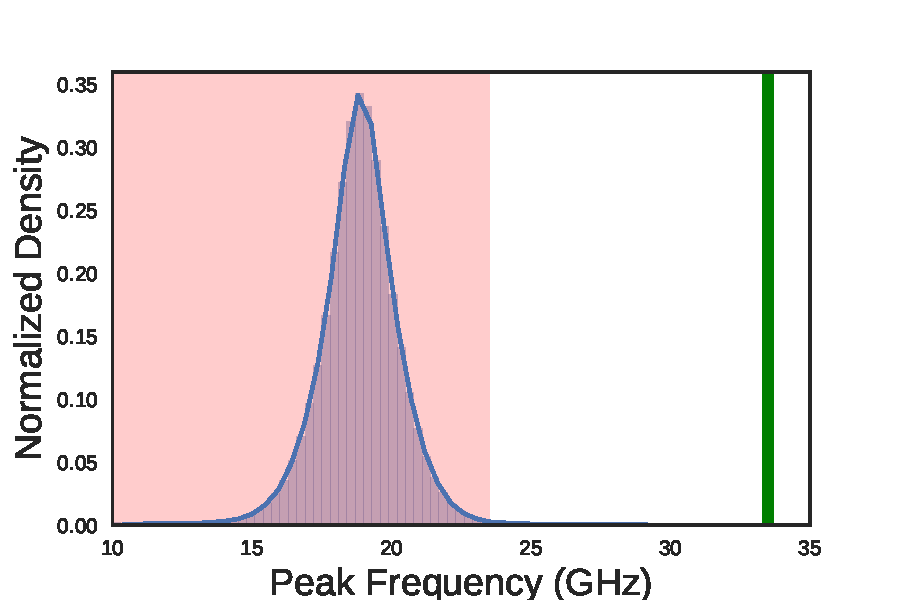
\includegraphics[width=\textwidth]{../Plots/ch_intro/AME_commander_freqdist.pdf}
                \centering
                \caption{The peak frequencies of the varying component $AME_{var}$.  The pink shaded region indicates frequencies not covered by either WMAP or Planck The green line at 33.5~GHz indicates the peak frequency of $AME_{fix}$.}
                \label{fig:AME_commander_freqdist}
              \end{figure}
          Only the fitted global frequency, 33.5~GHz for the spatially constant component, is covered. However they note that the combined components, per pixel, would have an average peak  at least within the WMAP coverage range. In general, $AME_{var}$ is the dominant component, accounting for approximately 90\% of the total fitted AME intensity between 20 and 40~GHz, indicated by the full-sky histograms in Fig.~\ref{fig:AME_comps_distplot}.
              \begin{figure}
                 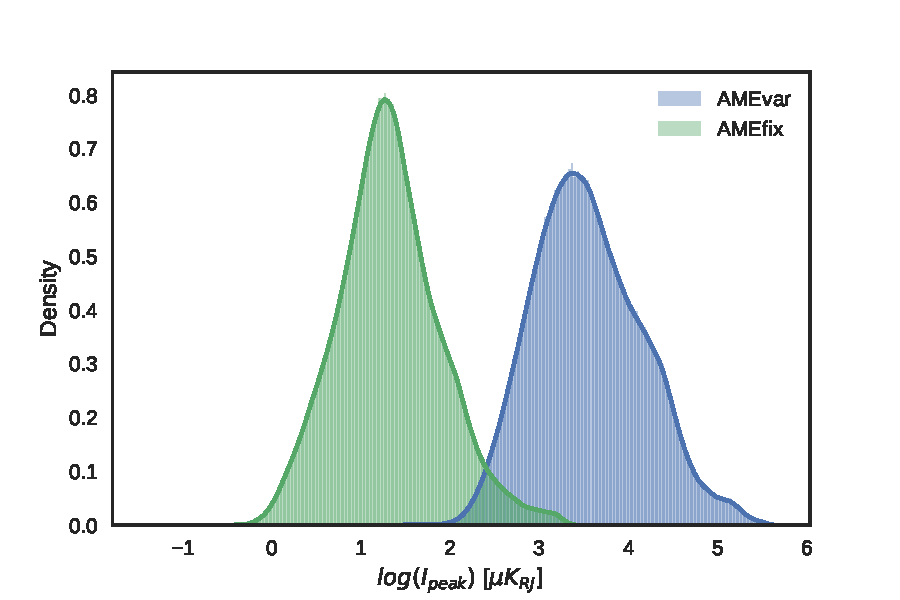
\includegraphics[width=\textwidth]{../Plots/ch_datasources/AME_comps_distplot.pdf}
                 \centering
                 \caption{Histograms of the peak intensity AME maps calculated from the original COMMANDER-AME reference frequency maps. The dominant component, $AME_{var}$ is indicated in blue, for all pixels in the map, with their spinning dust intensities evaluated their peak frequencies (see Fig.~\ref{fig:AME_commander_freqdist}.) $AME_{fix}$ gives the peak intensity of the spatially-constant frequency component, indicating it is essentially always the weaker component.}
                 \label{fig:AME_comps_distplot}
              \end{figure}
           As they are provided in PR2, the intensities are in fact the fitted spinning dust profiles for each pixel, evaluated at reference frequencies: 22.8~GHz for $AME_{var}$, 41~GHz for $AME_{fix}$ (for convenient comparison to the WMAP total intensity maps at those frequencies). Fig.~\ref{fig:AME_comps_distplot} in fact indicates our own re-evaluation of the fitted spinning dust SEDs at their peak frequencies, as the reference frequencies to not have any special physical relevance. This conversion does not have a significant effect on the results in the chapters to follow, except in the case of some outlying pixels with very low peak frequencies, easily seen in the map of the fitted frequencies in Fig.~\ref{fig:PCAME_var_freq}.
               \begin{figure}
                 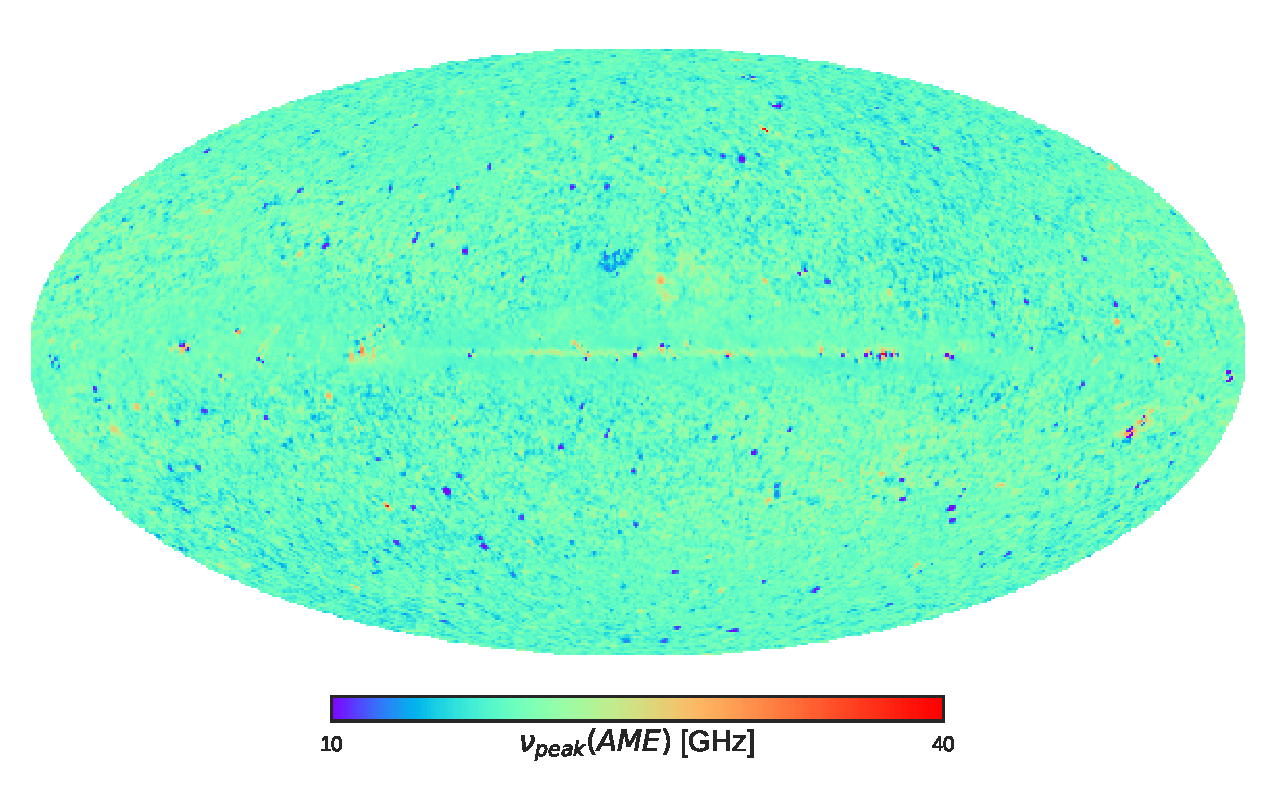
\includegraphics[width=\textwidth]{../Plots/ch_datasources/PCAME_var_freq.pdf}
                 \centering
                 \caption{All-sky map of the peak frequencies of the varying component $AME_{var}$, corresponding to Fig.~\ref{fig:AME_commander_freqdist}. Virtually all of the purple regions of the map correspond to pixels flagged for point sources in the LFI data. There are very few notable structures in the frequency map overall, other than the galactic plane itself, $\rho$~Ophiuchus, and Perseus.}
                 \label{fig:PCAME_var_freq}
               \end{figure}
            However on comparison to point source masks by Planck, we find that these outliers correspond to intensity outliers in the LFI 30~GHz map. This is not readily apparent when viewing the $AME_{var}$, evaluated at 22.8~GHz, as it is provided in \cite{planck15X}.

        \subsubsection{Spinning dust fitting}
          The actual spinning dust SED which is fitted to the Planck data by is indicated by Fig.~\ref{fig:AME_commander_freqshift_templ}, which we have reproduced from the original template provided in \cite{ali-haimoud09}.
              \begin{figure}
                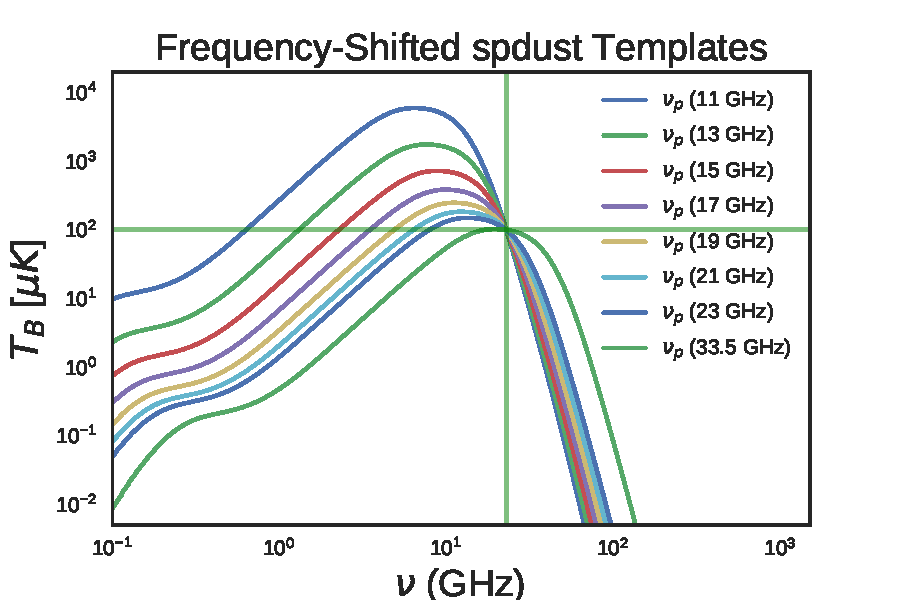
\includegraphics[width=\textwidth]{../Plots/ch_datasources/AME_commander_freqshift_templ.pdf}
                \centering
                \caption{Spdust template spinning dust profiles fitted by PC15X when calculating $AME_{var}$.  The reference frequency, 22.8~GHz is indicated by the vertical green line. Each template has the same $AME_{var}$ amplitude of 100~$\mu$K, indicated by the horizontal green line, plotted to highlight the potential deviation between $AME_{var}$ and the actual peak intensity. }
                \label{fig:AME_commander_freqshift_templ}
              \end{figure}
          PC15X fit the AME by applying a frequency shift and intensity shift parameter to this template. The physical parameters of the 'spdust' model itself are not directly varied in PC15X. In any case, the spinning dust model SED shape does not show significant variation from environment to environment \citep{ali-haimoud09}.
         Because of the phenenological approach of the AME fitting method, the PC15X authors themselves suggest caution in deriving conclusions from comparisons with the COMMANDE AME map. However it is the most thorough all-sky component separation currently available, and has not been well analyzed relative to the full wavelength range of available IR all-sky maps. Improving on the COMMANDER AME map will likely require lower frequency constraints (in the red-shaded portion of Fig.~\ref{fig:AME_commander_freqdist}) and/or higher resolution observations of not only the AME itself but the contribution from synchrotron and free-free emisson. This way some of the inherent degeneracies between free-free, synchrotron, thermal dust, and AME parameters may be able to be broken.
          \begin{figure}
               \centering
               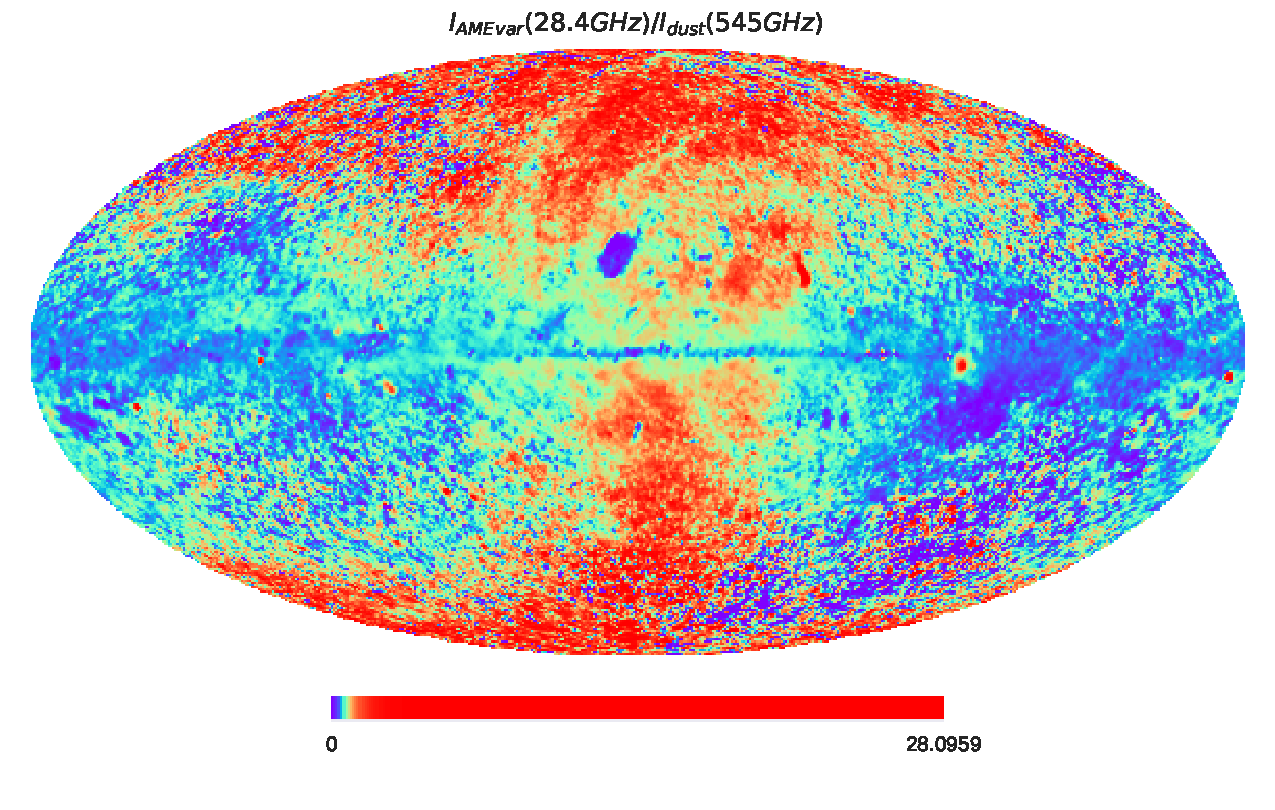
\includegraphics[width=\textwidth]{../Plots/ch_datasources/R_PCAMEtoPCRad.pdf}
               \caption{All-sky map of the ratio of two COMMANDER components- the frequency-varying AME component divided by the intensity of thermal dust emission at 545~GHz. There are some recognizable AME emission regions, such as $\lambda$~Orionis. Large-scale patches of AME excess are noted to correspond to synchrotron emission \citep{hensley16}}
               \label{fig:R_PCAMEtoPCdust}
           \end{figure}

  \section{All-sky Data Processing}

        The HFI, FIS, and IRIS maps used here are downloaded from their respective online repositories, as all-sky HEALPix\footnote{HEALPix core software is described at \url{http://healpix.sourceforge.net}. The HEALPIx python package {\tt healpy} used in this work is available at: \url{https://github.com/healpy/healpy}} maps \citep{gorski05}.   NSIDE~2048 maps. In the case of the IRC maps, we first create HEALPix maps from the 4,857 all-sky survey tiles using the Aladin all-sky data visualization platform \citep{bonnarel00}. NSIDE~2048 implies an average pixel spacing of 1.7$'$. The maps are then degraded to NSIDE~1024 before carrying out a Gaussian-beam smoothing to a 1$^{\circ}$ FWHM. Map smoothing itself is done in spherical harmonic space, before the maps and transformed back to position space. These steps are handled by the smoothing function contained in the {\tt healpy} python package. Following the smoothing process, the maps are degraded once more to NSIDE~256, or 15$'$ pixel-width \footnote{HEALPix pixel scale rebinning carried out with {\tt healpy.ud\_grade}}. The value of each of the larger NSIDE~256 pixels, comes from the mean of its parent NSIDE~1024 pixels. The purpose of this processing is to ensure that all of the maps have the same resolution as the PR2 AME map.
